\section{Introduction}

\begin{frame}{Introduction}
    Large Language Models (LLMs) are revolutionizing software development. Currently, they are used in a zero-shot manner: developers ask, and the assistant provides code. This limits their ability to handle complex tasks.

    \vspace{0.5cm}

    What if LLMs could iteratively test and improve their code? Can we enhance their potential by incorporating reasoning and domain-specific knowledge?

    \begin{figure}[!htb]
        \centering
        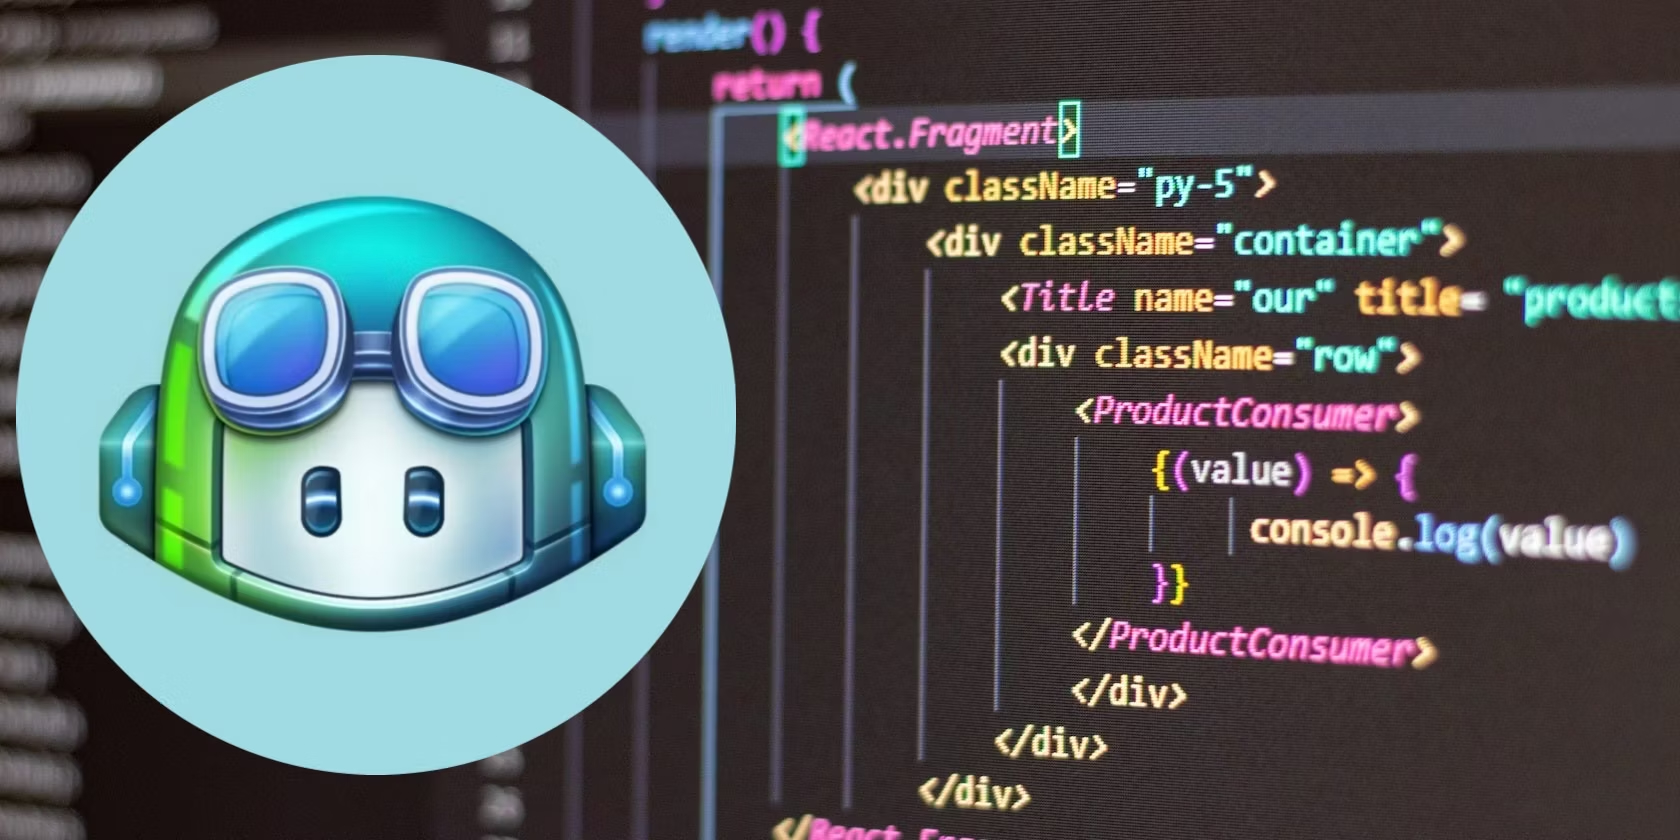
\includegraphics[width=0.5\textwidth]{img/llm_for_coding}
    \end{figure}
\end{frame}

\begin{frame}{Introduction}
    This thesis introduces \textbf{CoT-SelfEvolve}, a novel framework that further enhances self-correcting LLMs through:

    \begin{itemize}
        \item \textbf{Chain-of-Thought prompting} to guide LLM reasoning.
        \item \textbf{Integration of external knowledge} from StackOverflow to provide domain-specific context.
    \end{itemize}

    \begin{figure}[!htb]
        \centering
        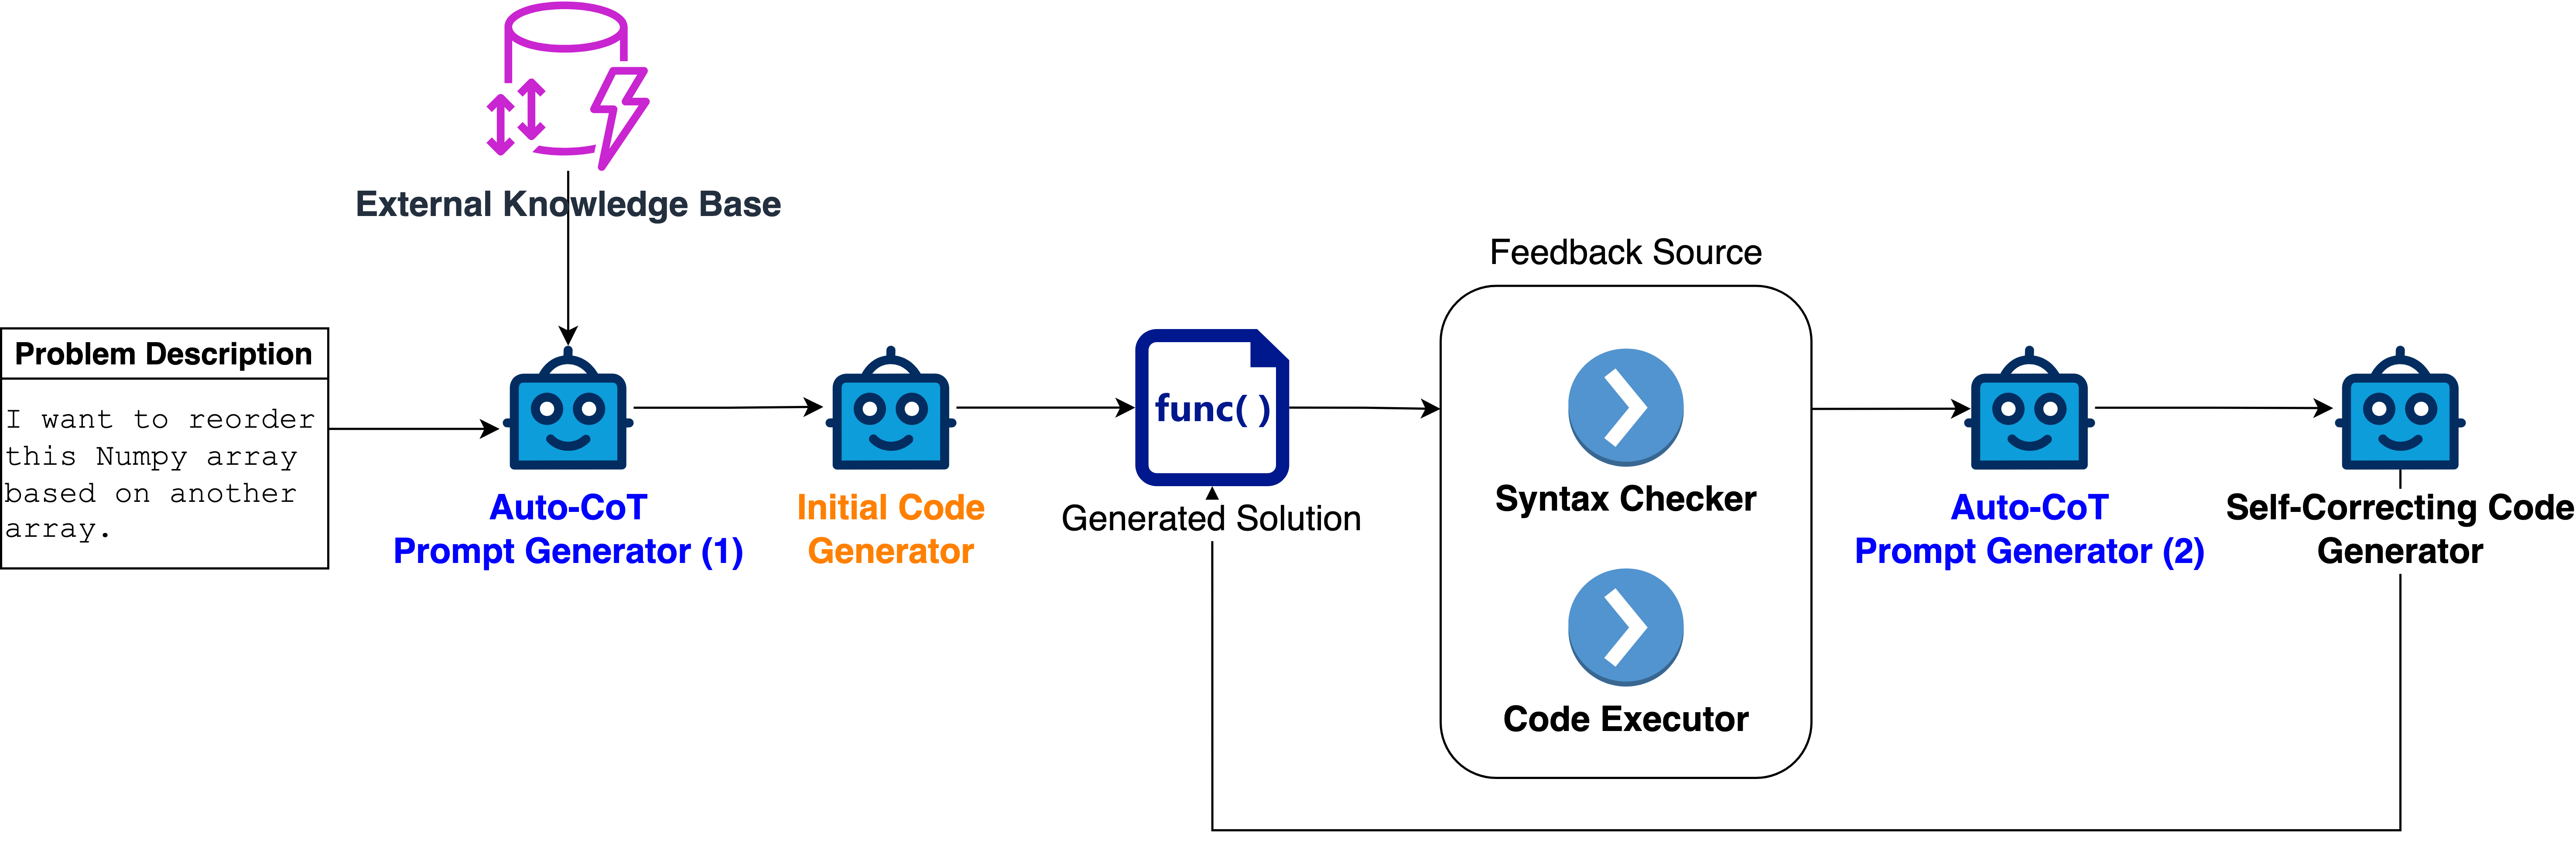
\includegraphics[width=0.8\textwidth]{img/cot_selfevolve_architecture}
        \captionsetup{font=small,labelformat=empty}
        \caption{Architecture of the CoT-SelfEvolve model (this study).}
    \end{figure}
\end{frame}
